\section{Methodology}
%This section outlines the methodology employed to evaluate the effectiveness of LLM-generated personalized POI descriptions compared to original manual descriptions. The study design, description personalization process, evaluation interface, metrics, procedure, and participant recruitment are described below.
This study examines how users perceive LLM-adapted POI descriptions in comparison to original, manually written descriptions. It focuses on perceived information quality, specifically clarity, trustworthiness, and relevance, rather than on recommendation accuracy or task performance. We conducted a user-centered comparative study in which participants evaluated paired descriptions of the same POI. Each pair included an original description sourced from existing online material and an LLM-adapted version personalized using the participant’s stated preferences. Participants were not informed which description was AI-generated, ensuring that evaluations reflected perceived qualities rather than source awareness.

\subsection{Study Design}
A within-subjects experimental design was employed in which each participant evaluated both original and AI-personalized descriptions for multiple POIs. This design enabled direct comparison between description types while controlling for individual differences in preferences and expectations. The study presented participants with 10 POIs spanning five categories (two per category): accommodation (Hotel Hassler Roma, The Savoy), natural attractions (Jungfraujoch, Neuschwanstein Castle), entertainment (Cologne Carnival, Cannstatter Volksfest), cultural and historical sites (Colosseum, Louvre Museum), and commercial destinations (Via del Corso, Caf\'{e} Central Vienna). POIs were selected to include both internationally recognized locations (e.g., Colosseum, Louvre) and regionally significant destinations (e.g., Cannstatter Volksfest), providing variety in familiarity levels.

\subsection{Participants}
A total of 51 participants were recruited through personal networks via email and direct messaging. Participants were required to be at least 18 years old and possess basic English proficiency to ensure effective engagement with POI descriptions. No specific travel experience was mandated, as the study aimed to assess AI-generated descriptions across diverse user segments.

Participants ranged from 22 to 49 years old ($\mu = 30.94$, $\sigma = 6.74$), with 67\% male and 33\% female. The sample was predominantly Indian (n = 28) and German (n = 21), with additional participants from China (n = 1) and Iran (n = 1). Professionally, participants included students (n = 22), engineers (n = 16), academics (n = 3), and other professions (n = 10). Most reported intermediate (n = 21) or experienced (n = 19) travel levels. The sample's geographic concentration reflects convenience sampling through personal networks rather than stratified recruitment; accordingly, findings should be interpreted as applicable to technology-familiar, educated populations with similar demographics.

\subsection{LLM-Based Personalization of POI Descriptions}
To operationalize personalization in the study, we employed a lightweight and explicit user profile derived from participants’ self-reported attributes and preferences. The profile was not intended as a predictive user model, but rather as a structured representation of personal context used to guide content adaptation. Personalization focused on adjusting emphasis and framing within POI descriptions while preserving their original meaning and factual content.

For each POI, two description versions were prepared. The original description was sourced from official tourism websites and travel platforms, representing standard, non-personalized content. The AI-adapted version was generated using gpt-4o-2024-11-20\footnote{\url{https://platform.openai.com/docs/models/gpt-4o}} with the default temperature setting. The model received a system prompt instructing it to act as an expert travel writer, emphasizing unique aspects, cultural significance, and visitor experience while adapting content to the user's situation. The user prompt included ten personalization dimensions: age, gender, marital status, whether the user has children, interests, travel experience level, education, profession, hobbies, and preferred travel style. The original POI title and description were provided, and the model was instructed to maintain factual accuracy and length, while emphasizing aspects most relevant to the user's profile. To verify factual preservation, a subset of generated descriptions was manually reviewed during initial testing to confirm that no factual claims were altered or fabricated during personalization. For example, a museum description for a participant interested in history would emphasize historical significance and artifacts, while the same museum described for a family traveler would highlight interactive exhibits and educational programs.

\subsection{Evaluation Interface}
Participants viewed descriptions through a web-based interface that displayed two versions side by side, labeled as Version A and Version B (see Figure~\ref{fig:eval-interface}). The interface did not indicate which version was AI-generated. Each POI was accompanied by a representative image to provide visual context. The presentation order of AI and manual descriptions was randomized across POIs to prevent order bias. Participants could not proceed to the next POI without completing evaluations for the current one, ensuring complete data collection.

\begin{figure*}[h]
  \centering
  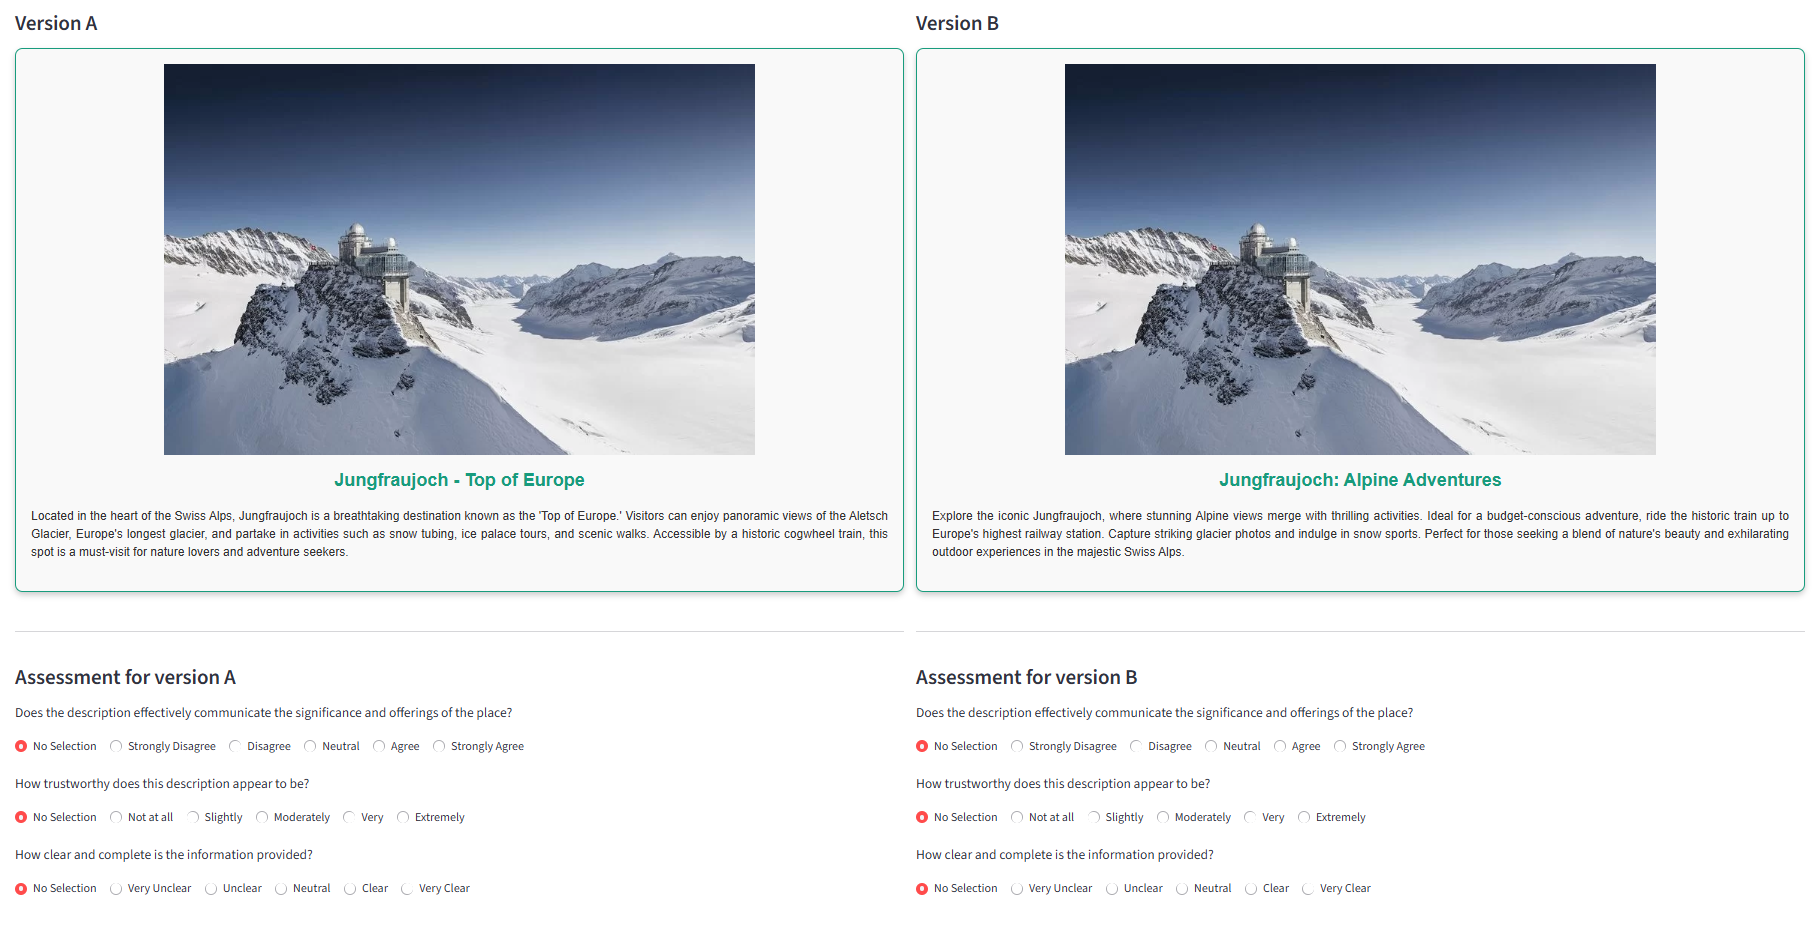
\includegraphics[width=0.90\linewidth]{figures/PoI_survey_img.png}
  \caption{Evaluation interface showing two description versions (Version A and Version B) presented side by side for participant comparison}
  \Description{Screenshot of the evaluation interface displaying two POI description versions with an image of Jungfraujoch mountain peak}
  \label{fig:eval-interface}
\end{figure*}

\subsection{Information Quality Measures}

Participants assessed each POI description along three perceptual dimensions using 5-point scales:
\begin{itemize}
    \item \textbf{Significance}: ``Does the description effectively communicate the significance and offerings of the place?'' (5-point agreement scale: 1 = Strongly Disagree, 5 = Strongly Agree)
    \item \textbf{Trustworthiness}: ``How trustworthy does this description appear to be?'' (5-point intensity scale: 1 = Not at all, 5 = Extremely)
    \item \textbf{Clarity}: ``How clear and complete is the information provided?'' (5-point clarity scale: 1 = Very Unclear, 5 = Very Clear)
\end{itemize}

After rating both descriptions individually, participants completed comparative judgments indicating which description was more engaging, informative, appealing, and more likely to encourage a visit. Participants also reported their prior familiarity with each POI (visited, heard of, or unfamiliar).


%\subsection{Statistical Analysis}
%Results are summarized using mean ratings across all POIs and participants ($N = 510$ paired observations per metric). Because each participant evaluated both manual and AI-adapted descriptions for the same POI, paired statistical tests were employed to account for the within-subjects design. Specifically, paired $t$-tests assessed mean differences under the assumption of normally distributed difference scores, while Wilcoxon signed-rank tests provided a non-parametric alternative that does not assume normality. Both tests were applied to each metric (significance, trustworthiness, and clarity) to ensure robustness of conclusions. Statistical significance was evaluated at $\alpha = 0.05$.

\subsection{Procedure}
The study was conducted in three phases using a secure web platform.  First, participants reviewed an informed consent form explaining the study purpose, voluntary participation, and data confidentiality. After providing consent, they completed a demographic and preference survey collecting age, gender, nationality, profession, current city, hobbies, preferred travel styles, and tourism interests. This information formed the basis for personalizing AI-generated descriptions. The interface required a minimum number of preference selections to ensure sufficiently expressive profiles. Based on this information, POI descriptions were automatically generated using a large language model in subsequent pages of the study.

Participants then proceeded to the main evaluation phase, where they were presented with POI descriptions adapted using their profile information alongside original descriptions. The adapted descriptions were generated dynamically after the profiling step and before the evaluation, without further user interaction. Second, participants evaluated 10 POIs sequentially by reading both description versions and rating them on core metrics and familiarity. This evaluation phase lasted approximately 20 to 30 minutes. Finally, participants provided overall feedback on their experience and their comfort level with AI-generated travel content. All data were collected anonymously to ensure privacy. The study was conducted in accordance with institutional ethical guidelines, with participants providing informed consent before participation.
% The study proceeded in three phases. First, participants reviewed an informed consent form explaining the study purpose, voluntary participation, and data confidentiality. After providing consent, they completed a demographic and preference survey collecting age, gender, nationality, profession, current city, hobbies, preferred travel styles, and tourism interests. This information formed the basis for personalizing AI-generated descriptions.

% Second, participants entered the main evaluation phase, viewing 10 POIs sequentially. For each POI, they read both description versions, rated each individually on the three core metrics, completed comparative evaluations, and indicated their familiarity with the location. The entire evaluation phase took approximately 20 to 30 minutes.

% Third, upon completing all POI evaluations, participants provided overall feedback rating their experience with the study, their opinion on automated description adaptation, and their comfort level with AI-generated travel content. All responses were collected anonymously through a secure web platform, ensuring participant privacy and compliance with ethical research standards.


